\bibliographystyle{csn690}
\bibliography{bibliography}

%\cleardoublepage
%\listoflistings
%\addcontentsline{toc}{chapter}{Seznam algoritmů}

%\cleardoublepage
%\listoffigures

\appendix

\cleardoublepage
\chapter{Obrazová příloha}
	\begin{figure}				
		\centering
		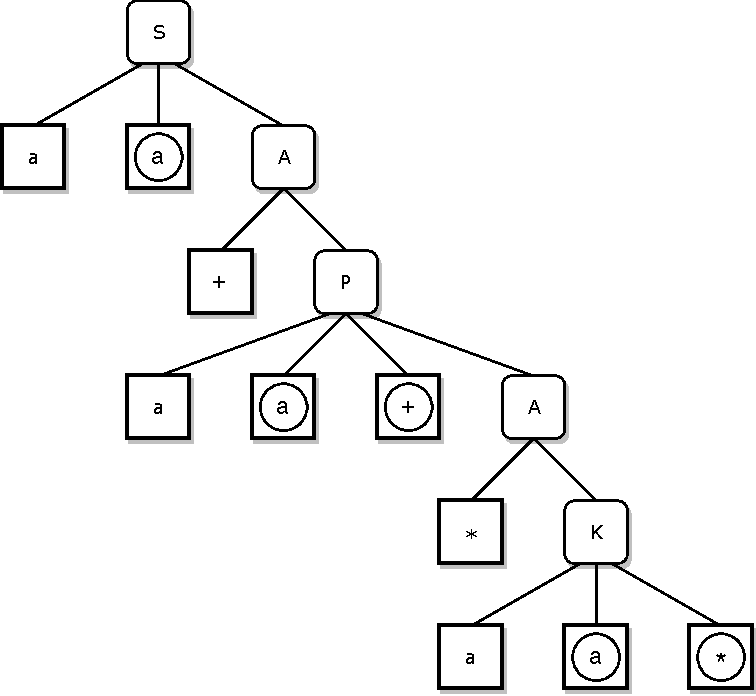
\includegraphics[width=0.8\linewidth]{img/PrekladovaGramatika}
		\caption{Ukázka překladové gramatiky}
		\label{fig:translateGrammar}
	\end{figure}
	\begin{figure}				
		\centering
		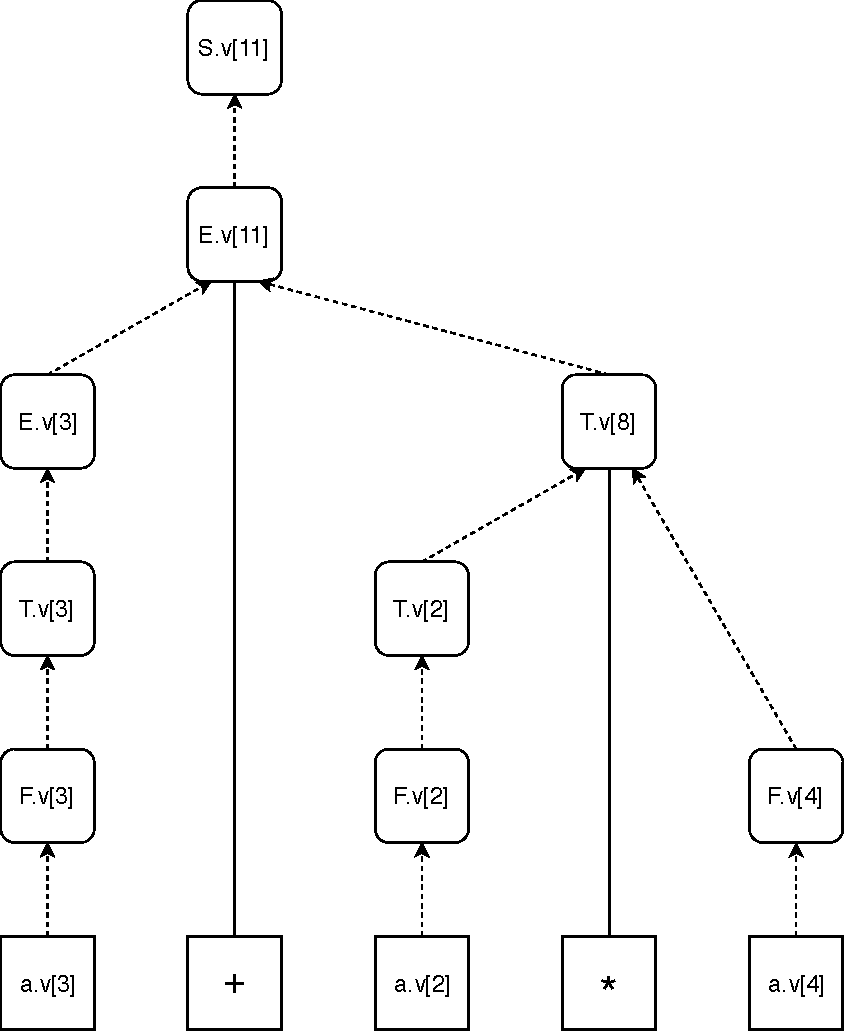
\includegraphics[width=0.8\linewidth]{img/AttributedArithmetic}
		\caption{Vyhodnocení atributů u atributované gramatiky}
		\label{fig:attributedGrammar}
	\end{figure}

	\begin{figure}				
		\centering
		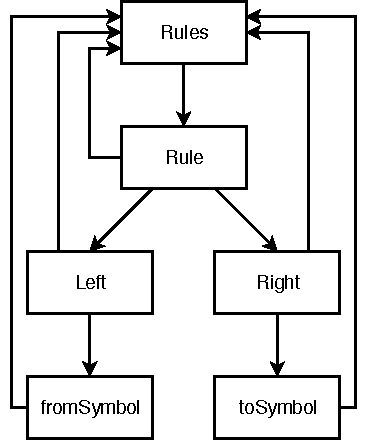
\includegraphics[width=0.4\linewidth]{img/RuleComputing}
		\caption{Výpočet vlastností pro třídu \Code{Rule}}
		\label{fig:ruleComputing}
	\end{figure}

	\begin{figure}				
		\centering
		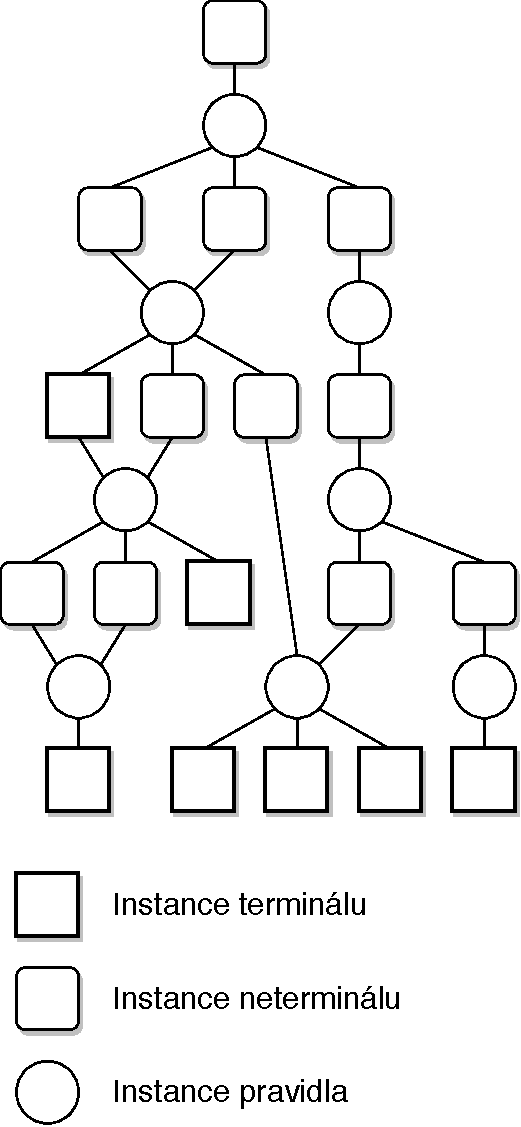
\includegraphics[width=0.6\linewidth]{img/Type0parsing}
		\caption{Reprezentace syntaktického stromu pro neomezené gramatiky}
		\label{fig:type0Parsing}
	\end{figure}

	\begin{figure}				
		\centering
		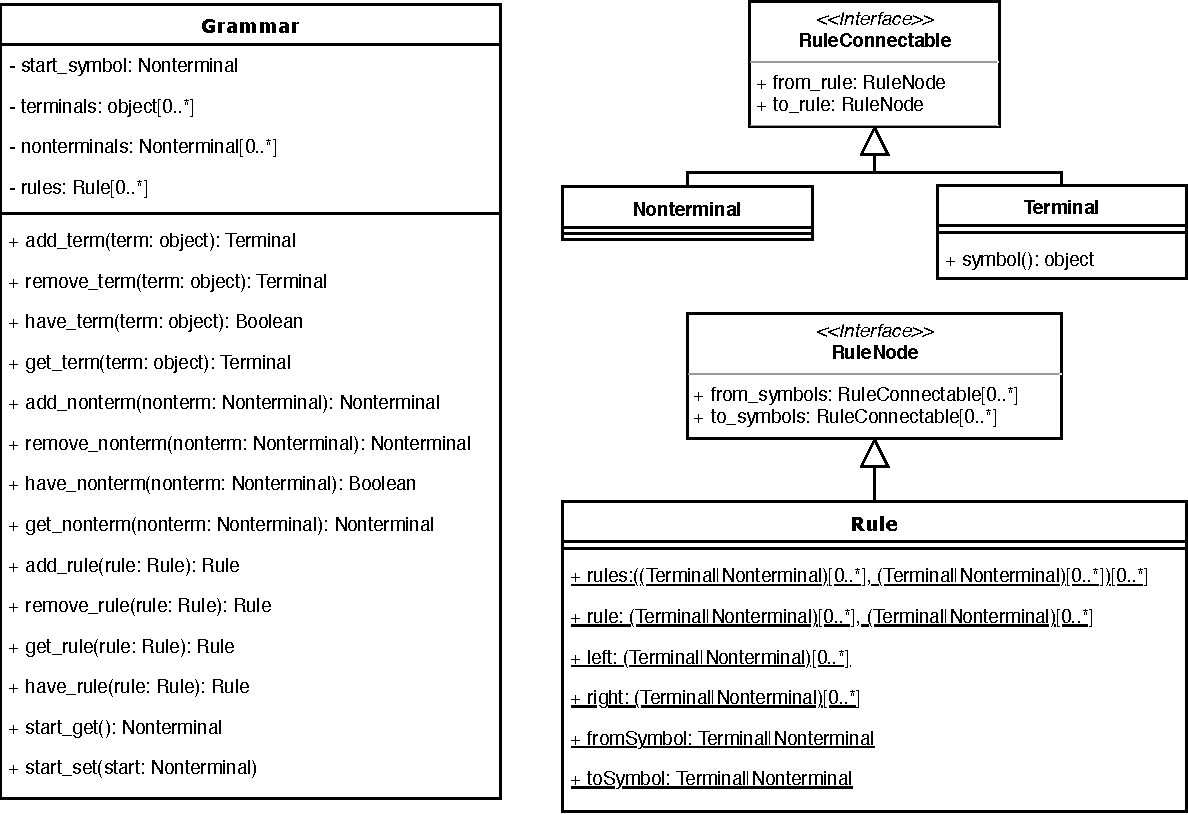
\includegraphics[width=0.9\linewidth]{img/WholeGrammpy}
		\caption{Kompletní návrh reprezentující gramatiku}
		\label{fig:grammpyWhole}
	\end{figure}

	\begin{figure}				
		\centering
		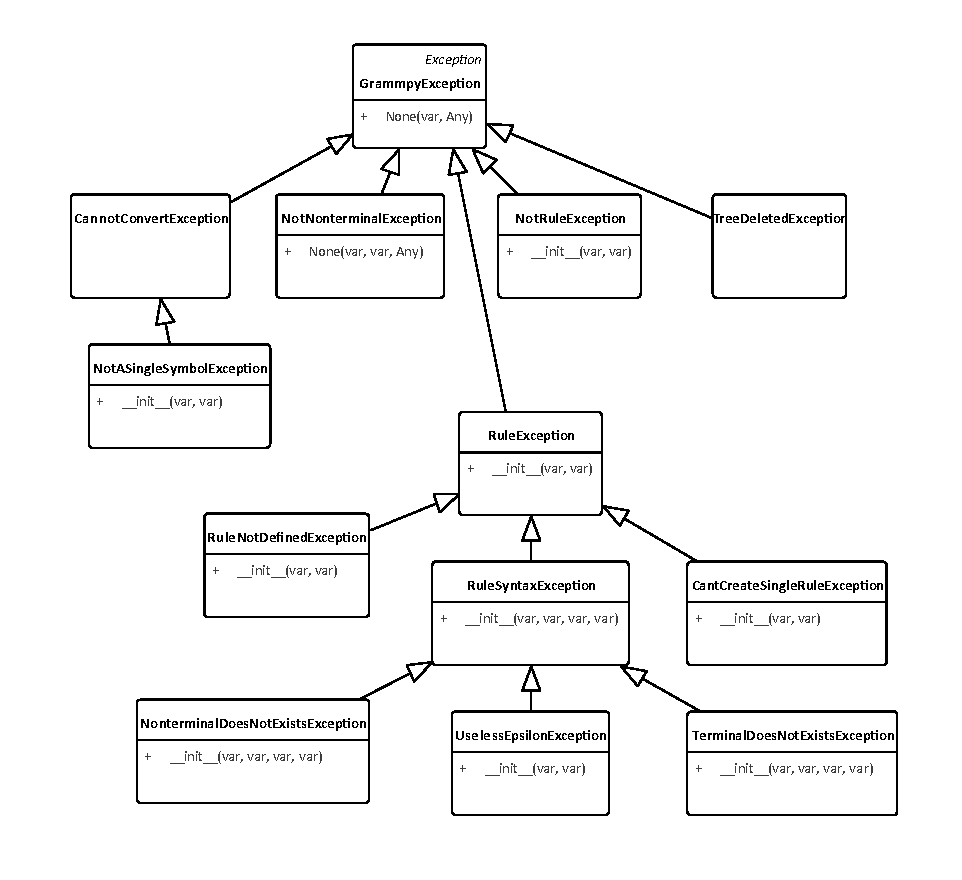
\includegraphics[width=0.8\linewidth]{img/grammpyExceptions}
		\caption{Hiearchie vyjímek v~modulu grammpy}
		\label{fig:grammpyExceptions}
	\end{figure}

	\begin{figure}				
		\centering
		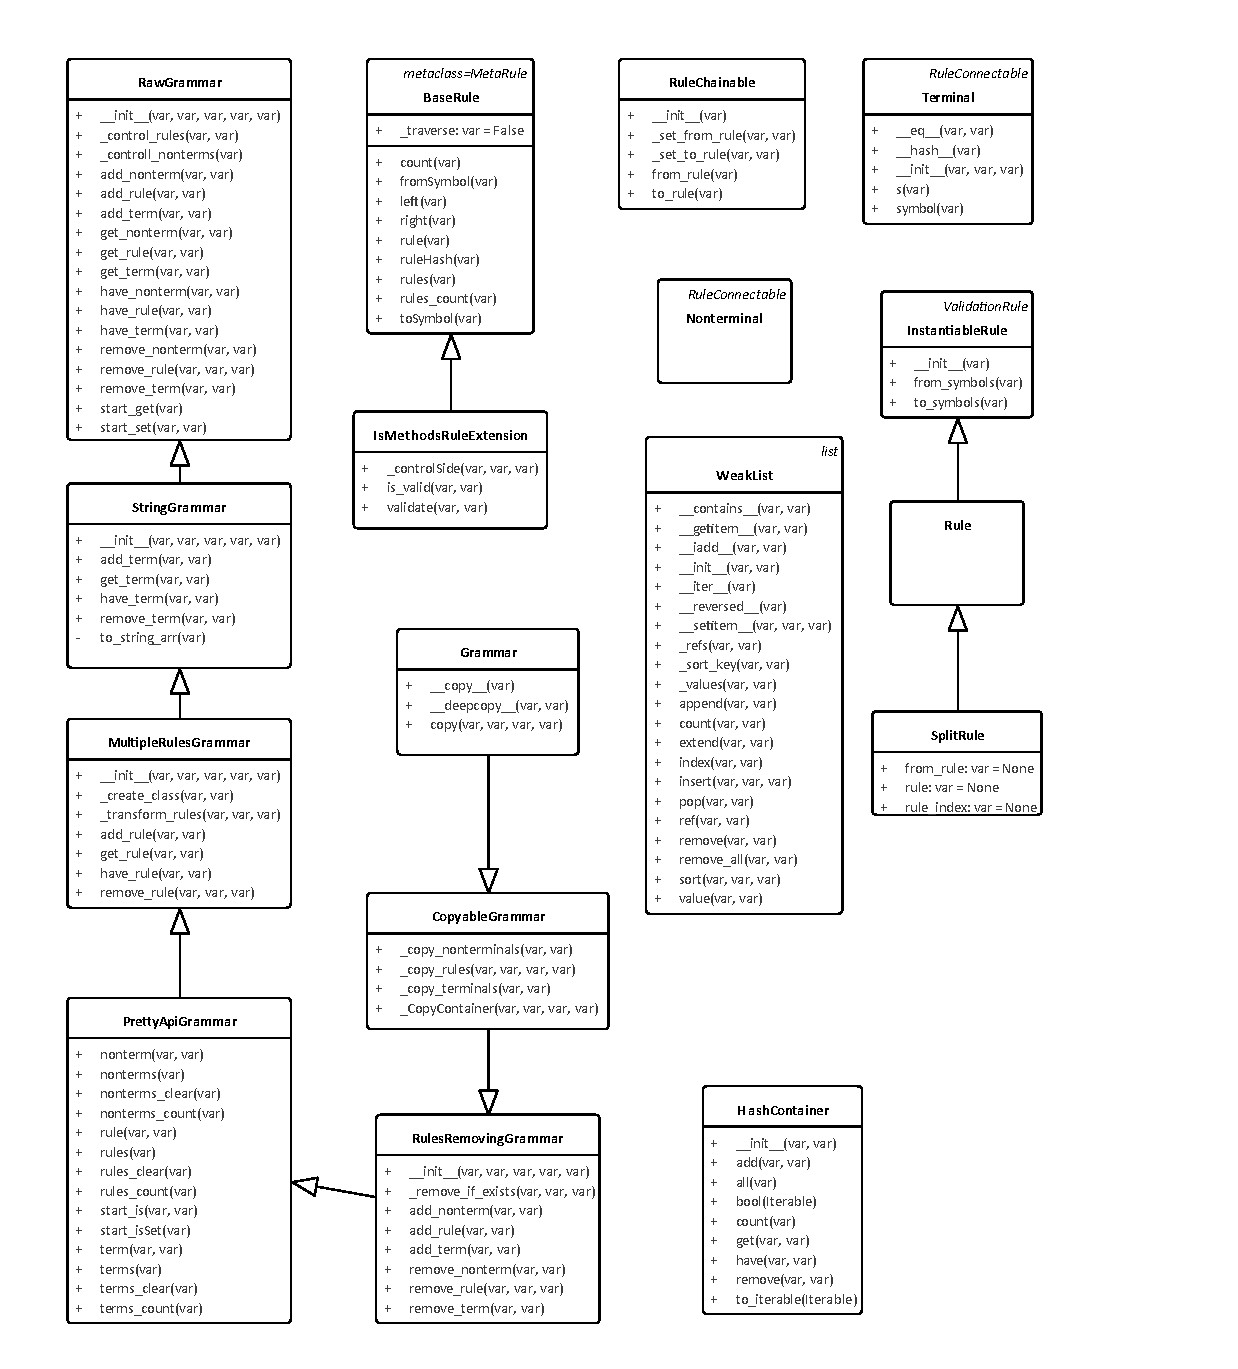
\includegraphics[width=\linewidth]{img/grammpyAPI}
		\caption{Class diagram implementace modulu grammpy}
		\label{fig:grammpyClasses}
	\end{figure}

	\begin{figure}				
		\centering
		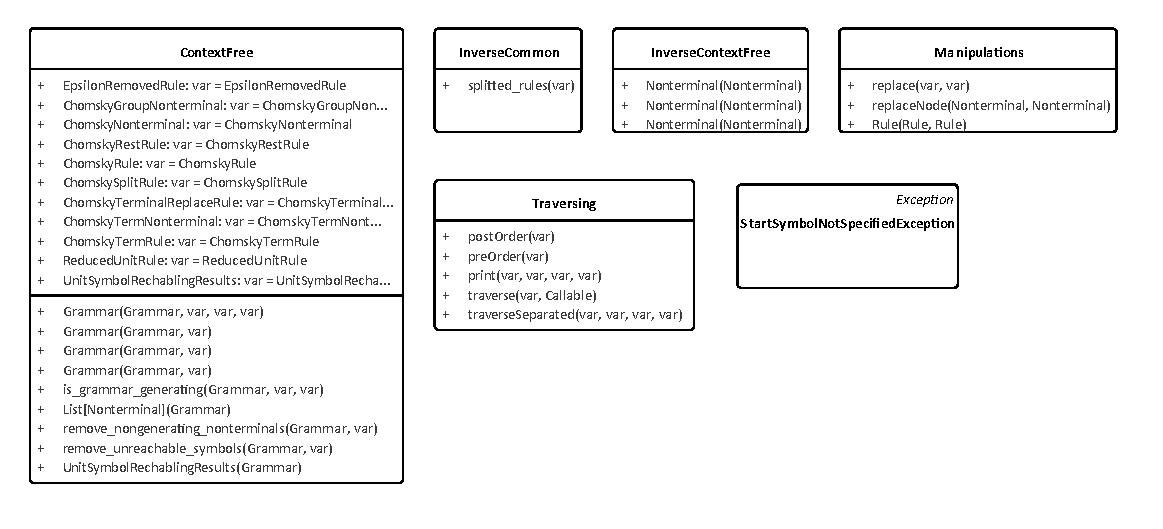
\includegraphics[width=\linewidth]{img/grammpy-transformsAPI}
		\caption{Class diagram implementace modulu grammpy-transforms}
		\label{fig:grammpyTransformsClasses}
	\end{figure}

	\begin{figure}				
		\centering
		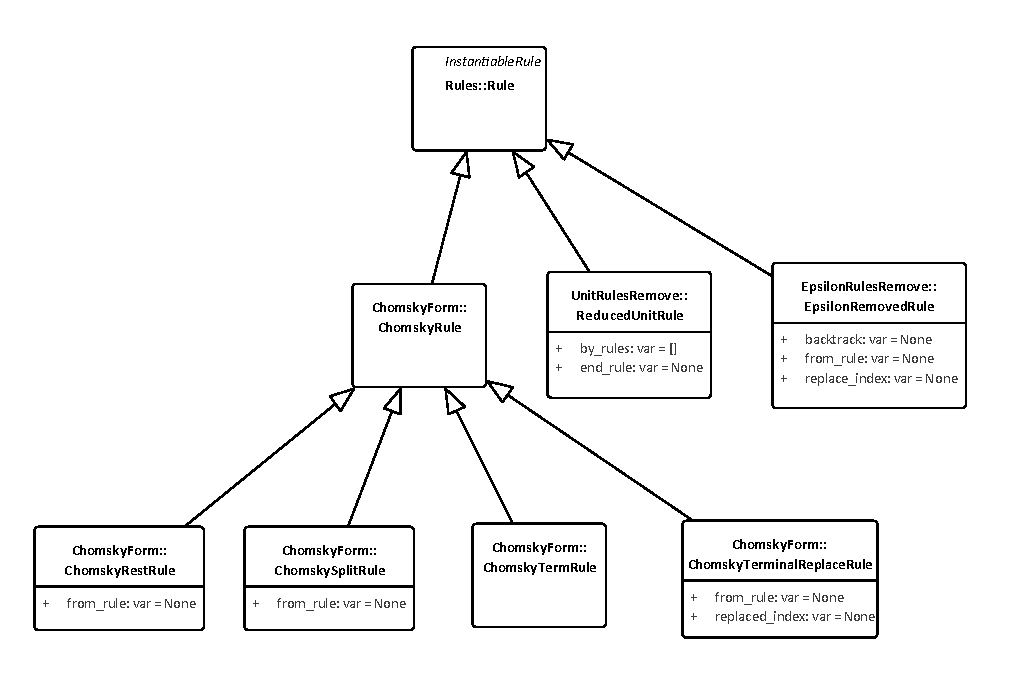
\includegraphics[width=0.8\linewidth]{img/grammpy-transformsRules}
		\caption{Class diagram pravidel v modulu grammpy-transforms}
		\label{fig:grammpyTransformsRules}
	\end{figure}

	\begin{figure}				
		\centering
		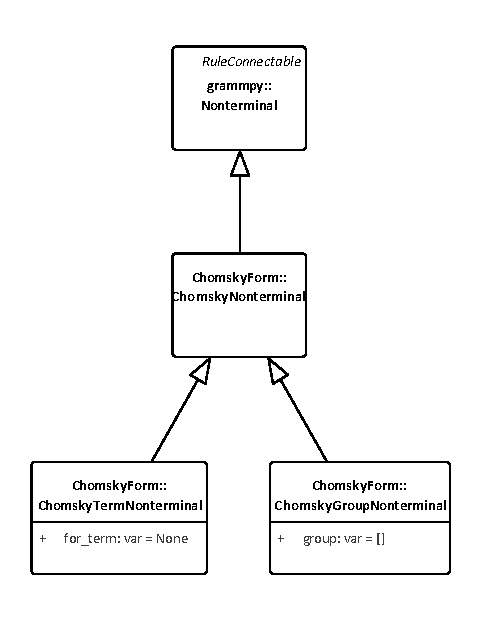
\includegraphics[width=0.4\linewidth]{img/grammpy-transformsNonterminals}
		\caption{Class diagram neterminálů v modulu grammpy-transforms}
		\label{fig:grammpyTransformsNonterminals}
	\end{figure}


\cleardoublepage
\printglossary[title=Seznam použitých zkratek]

\cleardoublepage
\chapter{Obsah přiloženého CD}
	\begin{figure}
		\dirtree{%
			.1 readme.txt\DTcomment{stručný popis obsahu CD}.
			.1 src.
				.2 grammpy\DTcomment{zdrojové kódy modulu grammpy}.
				.2 grammpy-transforms\DTcomment{zdrojové kódy modulu grammp-transforms}.
				.2 pyparsers\DTcomment{zdrojové kódy modulu pyparsers}.
			.1 examples\DTcomment{zdrojové kódy ukázek}.
				.2  lambda--cli\DTcomment{lambda kalkulus interpret}.
				.2  regex\_inverse\DTcomment{parser regulárních výrazů}.
				.2  calc\DTcomment{parser matematických výrazů}.
			.1 BP\_Valkovic\_Patrik\_2018.pdf\DTcomment{text práce ve formátu PDF}.
			.1 thesis\DTcomment{zdrojové soubory práce ve formátu \LaTeX}.
		}
	\end{figure}